% ---
% filename : nibt_installations_20260517_543_protection_salle_bains.tex
% id : nibt_installations_20260517_543
% title : "Degré de protection et installation en salle de bains"
% domain : "Nibt"
% subdomain : "Installations"
% tags : ["nibt", "salle_de_bains", "ip", "volume", "sécurité", "dt"]
% difficulty : 2
% time_solve : 15
% has_octave : false
% author : "om"
% ---
\documentclass[a4paper,11pt,answers,addpoints]{exam}
% ---------------------------------------------------------
% LANGUE, ENCODAGE, FONTS
% ---------------------------------------------------------
\usepackage[utf8]{inputenc}
% ---------------------------------------------------------
% GÉOMÉTRIE ET MISE EN PAGE
% ---------------------------------------------------------
\usepackage[left=1.7cm,right=1.5cm,top=2cm,bottom=1cm]{geometry}
\usepackage{microtype}
\usepackage{float}
\usepackage{needspace}

% ---------------------------------------------------------
% MATHÉMATIQUES
% ---------------------------------------------------------
\usepackage{amsmath, amssymb, bm, esvect}

\newcommand{\V}{\overrightarrow}
\def\vect#1{\overrightarrow{\strut#1}}
\providecommand{\Degrees}[0]{\ensuremath{^\circ}}

% ---------------------------------------------------------
% UNITÉS ET GRANDEURS (SIunitx)
% ---------------------------------------------------------
\usepackage{siunitx}
\sisetup{output-decimal-marker={,}}
\DeclareSIUnit \var {var}
\DeclareSIUnit \VA {VA}
\DeclareSIUnit \kVA {kVA}
\DeclareSIUnit[quantity-product={}] \degree{\text{\textdegree}}

% Permet la césure dans les nombres avec unités (évite les Underfull \hbox)
%\AllowBreakAtQQ

% ---------------------------------------------------------
% GRAPHIQUES : TikZ + CircuitikZ (sans tkz-fct qui cause des erreurs spath3)
% ---------------------------------------------------------
\usepackage{tikz}
\usetikzlibrary{
	arrows.meta,
	intersections,
	decorations.pathreplacing,
	%	positioning
}

\usepackage[european,straightvoltages,EFvoltages]{circuitikz}
\usepackage{pgfplots}
\pgfplotsset{compat=1.12}

% Symbole étoile-triangle personnalisé
\newcommand{\wye}{%
	\mathbin{\tikz[x=1ex,y=1ex]{%
			\draw[line width=.1ex] (0,0)--(45:1)--++(-45:1) (45:1)--++(0,1);
	}}%
}

% ---------------------------------------------------------
% TABLEAUX
% ---------------------------------------------------------
\usepackage{tabularx}
\usepackage{tabu}

% ---------------------------------------------------------
% HYPERLIENS
% ---------------------------------------------------------
\usepackage[colorlinks=true,
menucolor=red,
breaklinks=true,
urlcolor=blue,
linkcolor=blue]{hyperref}

% ---------------------------------------------------------
% COMMANDES PERSONNELLES
% ---------------------------------------------------------
\newcommand\nomauteur{bdminasmorgul@protonmail.com}
\newcommand\dateTe{18.05.2026}
\newcommand\brancheTe{DT}

% ---------------------------------------------------------
% STYLE DE L'EXERCICE
% ---------------------------------------------------------
\pagestyle{headandfoot}
\firstpageheadrule
\runningheadrule

% En-tête avec largeur fixe pour éviter les dépassements
\firstpageheader{\brancheTe\ (\nomauteur)}{Élève : }{\makebox[3.5cm][r]{\dateTe\ \thepage/\numpages}}
\runningheader{\brancheTe\ (\nomauteur)}{Élève : }{\makebox[3.5cm][r]{\dateTe\ \thepage/\numpages}}

% Pied de page
\newcommand{\totalpointtts}{%
	\begin{tikzpicture}[remember picture, overlay]
		\node[anchor=south west, inner sep=0pt, outer sep=0pt]
		at ([xshift=0.5cm,yshift=0.5cm]current page.south west)
		{\rotatebox{90}{Total des points : \numpoints}};
	\end{tikzpicture}%
}

\firstpagefooter{\hspace*{\fill}\totalpointtts}{}{}
\runningfooter{\hspace*{\fill}\totalpointtts}{}{}

% Réglages exam
\printanswers
\addpoints
\pointsinmargin
\bracketedpoints

% ---------------------------------------------------------
% LISTINGS (code)
% ---------------------------------------------------------
\usepackage{xcolor}
\usepackage{listings}

\lstdefinestyle{octavestyle}{
	language=Matlab,
	basicstyle=\ttfamily\small,
	keywordstyle=\color{blue},
	commentstyle=\color{green!50!black},
	stringstyle=\color{red},
	stepnumber=1,
	frame=single,
	breaklines=true,
	breakatwhitespace=true,
	tabsize=4
}

\usepackage{enumitem}
\setlist[enumerate,1]{label=\alph*), ref=\alph*)}
\newenvironment{explication}{%
	\par\noindent\textbf{Explication. }\itshape
}{\par\normalfont}

\begin{document}
	\unframedsolutions
	\pointsinmargin
	\bracketedpoints
	
\section*{Préparation DT PQ CFC ELMO,IELE,PELE}
\begin{questions}
\question
En tant qu'installateur-électricien, vous intervenez pour la pose d'un luminaire dans la salle de bains d'une villa. Le luminaire doit être fixé au plafond, verticalement au-dessus de la baignoire, dans une zone définie comme le volume \num{1}  selon la NIBT.
\begin{figure}[ht]
	\centering
	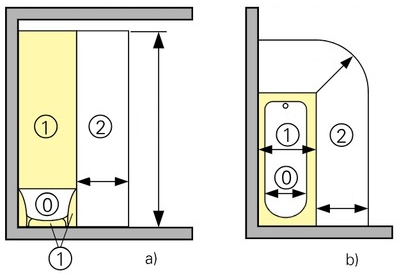
\includegraphics[scale=0.8]{volumes_0_1_2_Q.jpg}
\end{figure}
\begin{parts}
	\part[1] Quel est le degré de protection IP minimal requis pour ce luminaire, s'il n'y a pas de risque de jets d'eau~?
	\part[1] Quelle est la hauteur minimale de montage à respecter pour ce luminaire par rapport au sol fini pour rester conforme aux limites du volume \num{1}~?
	\part[1] Quel dispositif de protection complémentaire est impérativement requis pour l'ensemble des circuits de la salle de bains~?
	\part[1] Est-il autorisé d'installer une prise \qty{230}{[\volt]} à l'intérieur du volume \num{1} ou du volume \num{2}~?
\end{parts}

\begin{solution}\\
	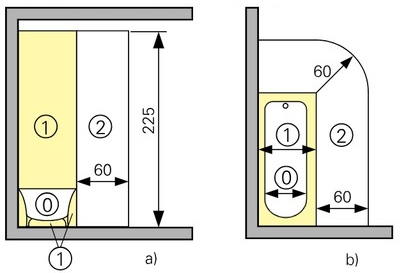
\includegraphics[scale=0.5]{volumes_0_1_2_rep.jpg}

	\begin{itemize}
		\item \textbf{Degré de protection} : NIBT 7.01.5.1.2.2,  Pour un luminaire situé en volume \num{1}, sans risque de jets d'eau, le degré de protection minimal est IP X4.
		\item \textbf{Hauteur de montage} : La limite supérieure du volume \num{1} est fixée à \qty{225}{[\centi\metre]} au-dessus du sol fini.
		\item \textbf{Protection complémentaire} : NIBT 4.1.1.3.3. Les prises librement accessibles avec un courant assigné $\leq \qty{32}{[\ampere]}$ doivent être protégées par un dispositif à courant différentiel-résiduel (DDR) avec $I_{\Delta n} \leq \qty{30}{[\milli\ampere]}$.
		\item \textbf{Appareillage} : Les socles de prises sont interdits dans les volumes \num{1} et \num{2}. Ils ne sont admis qu'en dehors du volume \num{2} (soit à plus de \qty{60}{[\centi\metre]} du bord de la baignoire).
	\end{itemize}
	
	Synthèse des valeurs de la NIBT~:
	\begin{align*}
		H_{\text{min\_volume1}} &= \qty{225}{[\centi\metre]} \\[6pt]
		IP_{\text{min\_V1}} &= \text{IP X4} \\[6pt]
		I_{\Delta n} &\leq \qty{30}{[\milli\ampere]} \\[6pt]
		D_{\text{prise\_min}} &> \qty{60}{[\centi\metre]} \text{ (hors volume 2)}
	\end{align*}
\end{solution}
\end{questions}
\end{document}